All 216 branches have completed. Figure~\ref{ca:fig:mv} shows the measured marginal value of
every provider on every domain at the four checkpoints.

\begin{figure}[htbp]
\centering
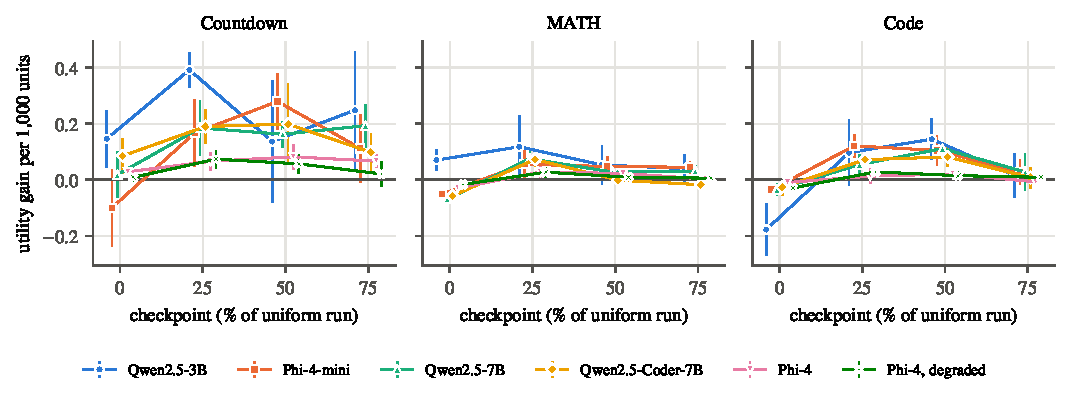
\includegraphics[width=\linewidth]{ca_marginal_value.pdf}
\caption{Marginal value: change in mean selection accuracy over the three domains after
20 rounds on one arm, per 1,000 price units, against the checkpoint the branch started
from. Points are means over three seeds and bars are $\pm 1$ standard error across seeds.
Points are offset horizontally for legibility.}
\label{ca:fig:mv}
\end{figure}

\paragraph{Per unit of budget, cheap providers lead.} On Countdown, the cheapest provider,
Qwen2.5-3B, has the highest mean marginal value at the 0, 25 and 75\% checkpoints, and
Phi-4-mini at 50\%. Qwen2.5-3B is the best Countdown arm in 8 of the 12 combinations of
seed and checkpoint. Per round, without dividing by price, the providers are much closer:
from the 25\% checkpoint, all six raise mean utility by between 0.022 and 0.033 in 20
Countdown rounds. Phi-4 teaches no faster per round, to within noise, than providers that
cost a third as much. It leads only on code from the untrained student, where every
provider lowered utility and Phi-4 lowered it least. The only differences that
are significant in paired comparisons within a seed all involve Phi-4: at 25\%, Qwen2.5-3B
beats Phi-4 and its degraded copy on Countdown, and Phi-4-mini beats Phi-4 on code.

\paragraph{H1 and H2 are not supported at this power.} The decision rules, fixed before the
runs, require the leading provider's 95\% interval to clear its rival's; here these are
t-intervals over the three seeds. With three seeds
this never happens between the cheap and mid-priced providers, at any checkpoint or in any
domain. The leading provider does change between checkpoints and domains, and rankings are
unstable (Kendall's $\tau$ between consecutive checkpoints ranges from $-0.60$ to $0.73$),
but changes of that size are also what noise alone would produce. On MATH and code, every
marginal value is close to zero, consistent with the pilot. The honest summary is that
provider value per unit of budget is dominated by price, that differences among the
affordable providers are smaller than this design can detect, and that H1 and H2 remain
open. Section~\ref{ca:sec:next} plans the measurements needed to settle them.
